\chapter{HASIL DAN PEMBAHASAN}
\label{chap:hasil-pembahasan}

Pada bab ini akan dijelaskan mengenai hasil implementasi
dan pengujian dari sistem \emph{provisioning} yang telah
dibuat sebelumnya pada bab 3. Pengujian yang dilakukan
menggunakan laptop penulis dan komputer dari laboratorium Rekayasa Perangkat
Lunak Teknik Informatika ITS. Spesifikasi dari laptop dan komputer
yang digunakan dapat dilihat pada tabel \ref{tb:spesifikasi-laptop-pengujian},
\ref{tb:spesifikasi-komputer-pengujian}, dan \ref{tb:spesifikasi-komputer-pengujian-2}.

\begin{longtable}{|c|c|}
  \caption{Spesifikasi Laptop untuk Pengujian}
  \label{tb:spesifikasi-laptop-pengujian} \\
  \hline
  OS     & Fedora Linux 42.20250614.0 (Kinoite) x86\_64 \\
  \hline
  Kernel & Linux 6.14.9-300.fc42.x86\_64                \\
  \hline
  CPU    & Intel(R) Core(TM) i7-10750H (12) @ 5.00 GHz       \\
  \hline
  Integrated GPU   & Intel UHD Graphics @ 1.15 GHz [Integrated]       \\
  \hline
  Discrete GPU    & NVIDIA GeForce GTX 1650 Ti Mobile [Discrete]       \\
  \hline
  RAM    & 15848MiB       \\
  \hline
\end{longtable}

\begin{longtable}{|c|c|}
  \caption{Spesifikasi Komputer Jenis Satu untuk Pengujian}
  \label{tb:spesifikasi-komputer-pengujian} \\
  \hline
  OS     & Ubuntu 24.04.2 LTS x86\_64 \\
  \hline
  Kernel & 6.11.0-26-generic          \\
  \hline
  CPU    & 12th Gen Intel i7-12700 (20) @ 4.800GHz       \\
  \hline
  GPU    & Intel AlderLake-S GT1       \\
  \hline
  RAM    & 31834MiB       \\
  \hline
\end{longtable}

\begin{longtable}{|c|c|}
  \caption{Spesifikasi Komputer Jenis Dua untuk Pengujian}
  \label{tb:spesifikasi-komputer-pengujian-2} \\
  \hline
  OS     & Ubuntu 24.04.2 LTS x86\_64 \\
  \hline
  Kernel & 6.11.0-24-generic          \\
  \hline
  CPU    & 12th Gen Intel i9-12900k (24) @ 5.100GHz       \\
  \hline
  GPU    & NVIDIA GeForce RTX 3080 Ti       \\
  \hline
  RAM    & 63998MiB       \\
  \hline
\end{longtable}

\section{Hasil Implementasi}
\label{sec:hasil-implementasi}

Subbab ini menjelaskan hasil implementasi yang dilakukan pada
Tugas Akhir.

\subsection{Implementasi Linux Bridge}
\label{subsec:implementasi-linux-bridge}

Linux \emph{bridge} yang telah dijelaskan sebelumnya dibuat
agar \emph{virtual machine} memiliki jangkauan alamat IP yang sama
dengan jangkauan alamat IP dari komputer \emph{host}. Jangkauan IP yang
sama dengan komputer \emph{host} diperlukan agar \emph{virtual machine}
yang berada di komputer A dapat berkomunikasi dengan \emph{virtual machine}
yang berada di komputer B.

Pada kode sumber \ref{cli:host-network-interface}, komputer \emph{host} memiliki
\emph{network interface} untuk ethernet bernama enp4s0. Linux \emph{bridge} yang
dibuat untuk implementasi tugas akhir ini adalah k3s-br0 dan enp4s0 menjadi
\emph{slave} dari Linux \emph{bridge} k3s-br0. Alamat IP dan jangkauan IP dari
komputer \emph{host} tersebut adalah 10.21.73.17 dengan \emph{subnet mask} /24
yang berarti dalam \emph{local area network} tersebut terdapat 255 alamat
IP yang dapat dibagikan oleh DHCP server.

{\renewcommand{\lstlistingname}{Instruksi Terminal}
\begin{lstlisting}[
  style=clistyle,
  caption={Informasi \emph{Network Interface} pada Komputer \emph{Host}},
  label={cli:host-network-interface}
]
...
2: enp4s0: <BROADCAST,MULTICAST,UP,LOWER_UP> mtu 1500 qdisc mq master k3s-br0 state UP group default qlen 1000
    link/ether c8:7f:54:6c:47:ff brd ff:ff:ff:ff:ff:ff
...
8: k3s-br0: <BROADCAST,MULTICAST,UP,LOWER_UP> mtu 1500 qdisc noqueue state UP group default qlen 1000
    link/ether 92:e9:0d:63:4e:32 brd ff:ff:ff:ff:ff:ff
    inet 10.21.73.107/24 brd 10.21.73.255 scope global dynamic noprefixroute k3s-br0
       valid_lft 94877sec preferred_lft 94877sec
    inet6 fe80::1d88:4787:24c3:2a99/64 scope link noprefixroute
       valid_lft forever preferred_lft forever
\end{lstlisting}
}

Agar \emph{virtual machine} memiliki jangkauan alamat IP yang sama dengan 
jangkauan alamat IP address yang didapat oleh komputer \emph{host}, \emph{virtual machine}
dapat menggunakan Linux \emph{bridge} yang sudah dibuat sebagai sumber jaringan
yang dipakai. Konfigurasi tersebut dapat dilakukan melalui konfigurasi berbentuk
xml seperti yang dapat dilihat pada kode sumber \ref{code:vm-interface-configuration}.
Alamat IP yang didapat pada \emph{virtual machine} dapat dilihat pada kode
sumber \ref{cli:vm-network-interface}.

\begin{lstlisting}[
  language=xml,
  style=codestyle,
  caption={Konfigurasi \emph{Interface} Jaringan pada \emph{Virtual Machine}},
  label={code:vm-interface-configuration}
]
...
<interface type='bridge'>
  <mac address='52:54:00:cf:ee:9e'/>
  <source bridge='k3s-br0'/>
  <model type='virtio'/>
  <alias name='net0'/>
  <address type='pci' domain='0x0000' bus='0x01' slot='0x00' function='0x0'/>
</interface>
...
\end{lstlisting}

{\renewcommand{\lstlistingname}{Instruksi Terminal}
\begin{lstlisting}[
  style=clistyle,
  caption={Informasi \emph{Network Interface} pada \emph{Virtual Machine}},
  label={cli:vm-network-interface}
]
...
2: enp1s0: <BROADCAST,MULTICAST,UP,LOWER_UP> mtu 1500 qdisc fq_codel state UP group default qlen 1000
    link/ether 52:54:00:cf:ee:9e brd ff:ff:ff:ff:ff:ff
    inet 10.21.73.134/24 brd 10.21.73.255 scope global dynamic noprefixroute enp1s0
       valid_lft 105859sec preferred_lft 105859sec
    inet6 fe80::5054:ff:fecf:ee9e/64 scope link proto kernel_ll
       valid_lft forever preferred_lft forever
...
\end{lstlisting}
}

Pada kode sumber \ref{cli:vm-network-interface}, alamat IP yang didapat oleh
\emph{virtual machine} adalah 10.21.73.134 dan memiliki \emph{subnet mask} /24.
Alamat IP dan \emph{subnet mask} yang didapat oleh \emph{virtual machine} sama
dengan alamat IP dan \emph{subnet mask} yang didapat oleh komputer \emph{host}.
Informasi lanjutan mengenai Linux \emph{bridge} dan \emph{network interfaces}
yang tersambung dapat dilihat pada kode sumber \ref{cli:bridge-interfaces}.

{\renewcommand{\lstlistingname}{Instruksi Terminal}
\begin{lstlisting}[
  style=clistyle,
  caption={Linux \emph{Bridge} dan \emph{Network Interfaces} yang Tersambung},
  label={cli:bridge-interfaces}
]
bridge name     bridge id               STP enabled     interfaces
k3s-br0         8000.92e90d634e32       yes             enp4s0
                                                        vnet7
\end{lstlisting}
}

Pada kode sumber \ref{cli:bridge-interfaces}, \emph{network interfaces} yang
berada di bawah Linux \emph{bridge} k3s-br0 adalah \emph{network interface}
enp4s0 dan vnet7. \emph{Network interface} enp4s0 merupakan \emph{network interface}
untuk ethernet sedangkan vnet7 merupakan \emph{virtual network} yang dibuat
dan tersambung dengan \emph{network interface} dari \emph{virtual machine}.
Gambaran mengenai hal tersebut dapat dilihat pada \ref{cli:vnet-big}.

\begin{lstlisting}[
  style=clistyle,
  caption={Hubungan Antar \emph{Devices}},
  label={cli:vnet-big}
]
VM's ethernet interface <-> vnet <-> Linux bridge <-> physical NIC
\end{lstlisting}

\subsection{Implementasi Cloud-init}
\label{subsec:implementasi-cloud-init}

Setiap \emph{virtual machine} yang dibuat memiliki sebuah \emph{file} berekstensi iso khusus
yang berisikan \emph{file} konfigurasi Cloud-init. \emph{File} tersebut kemudian akan digunakan
saat mendefinisikan konfigurasi xml dari \emph{virtual machine}. Contoh definisi konfigurasi
xml tersebut dapat dilihat pada kode sumber \ref{lst:xml-cloud-init}.

\lstinputlisting[
  language=go,
  style=codestyle,
  emphstyle=\color{black}\bfseries\underbar,
  emph={seedFile},
  caption={Konfigurasi xml dengan \emph{File} Cloud-init},
  label={lst:xml-cloud-init}
]{program/xml-cloud-init-iso.go}

Cloud-init yang berjalan pada \emph{virtual machine} menghasilkan \emph{file}
\emph{log} dari proses konfigurasi Cloud-init. \emph{File} tersebut dapat digunakan
untuk proses \emph{debug} konfigurasi yang digunakan. Cloud-init menghasilkan
dua \emph{file logging}, yaitu \emph{log} dari proses Cloud-init itu sendiri
dan \emph{log} dari \emph{command} yang dijalankan oleh Cloud-init. Hasil
dari dua \emph{file} tersebut dapat dilihat pada gambar \ref{fig:log-cloud-init}
dan gambar \ref{fig:log-output-cloud-init}.

\begin{figure}[H]
  \centering
  \fbox{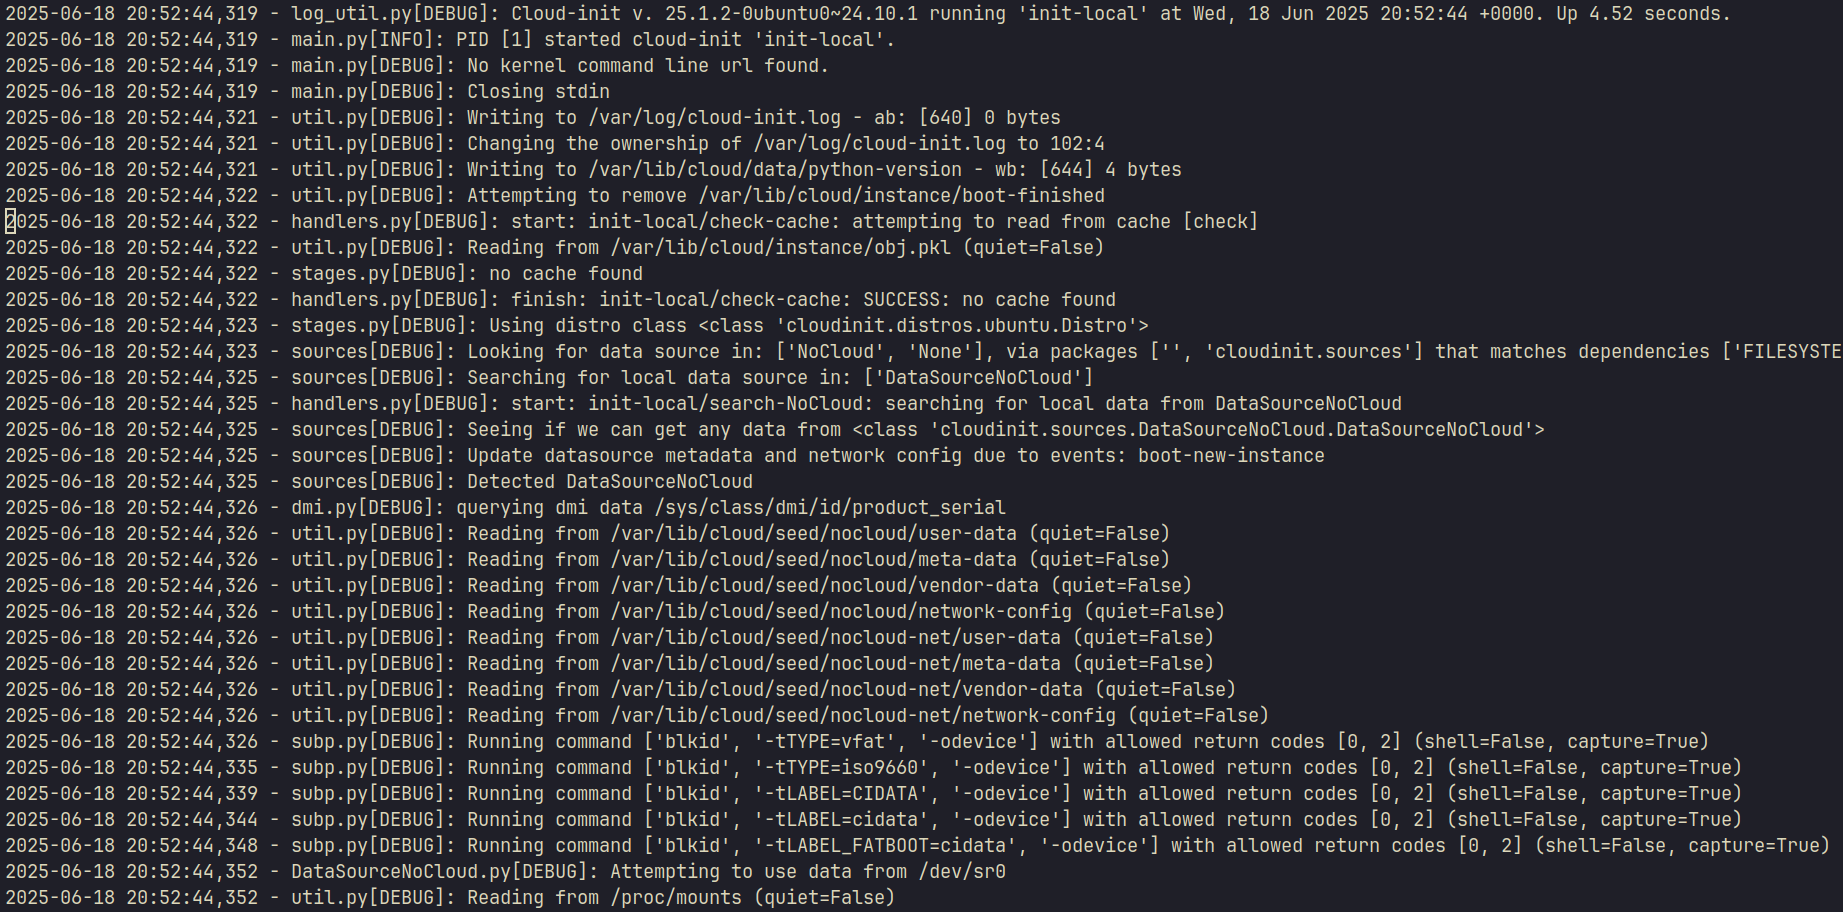
\includegraphics[scale=0.3]{gambar/cloud-init.png}}
  \caption{\emph{Log} Cloud-init}
  \label{fig:log-cloud-init}
\end{figure}

\begin{figure}[H]
  \centering
  \fbox{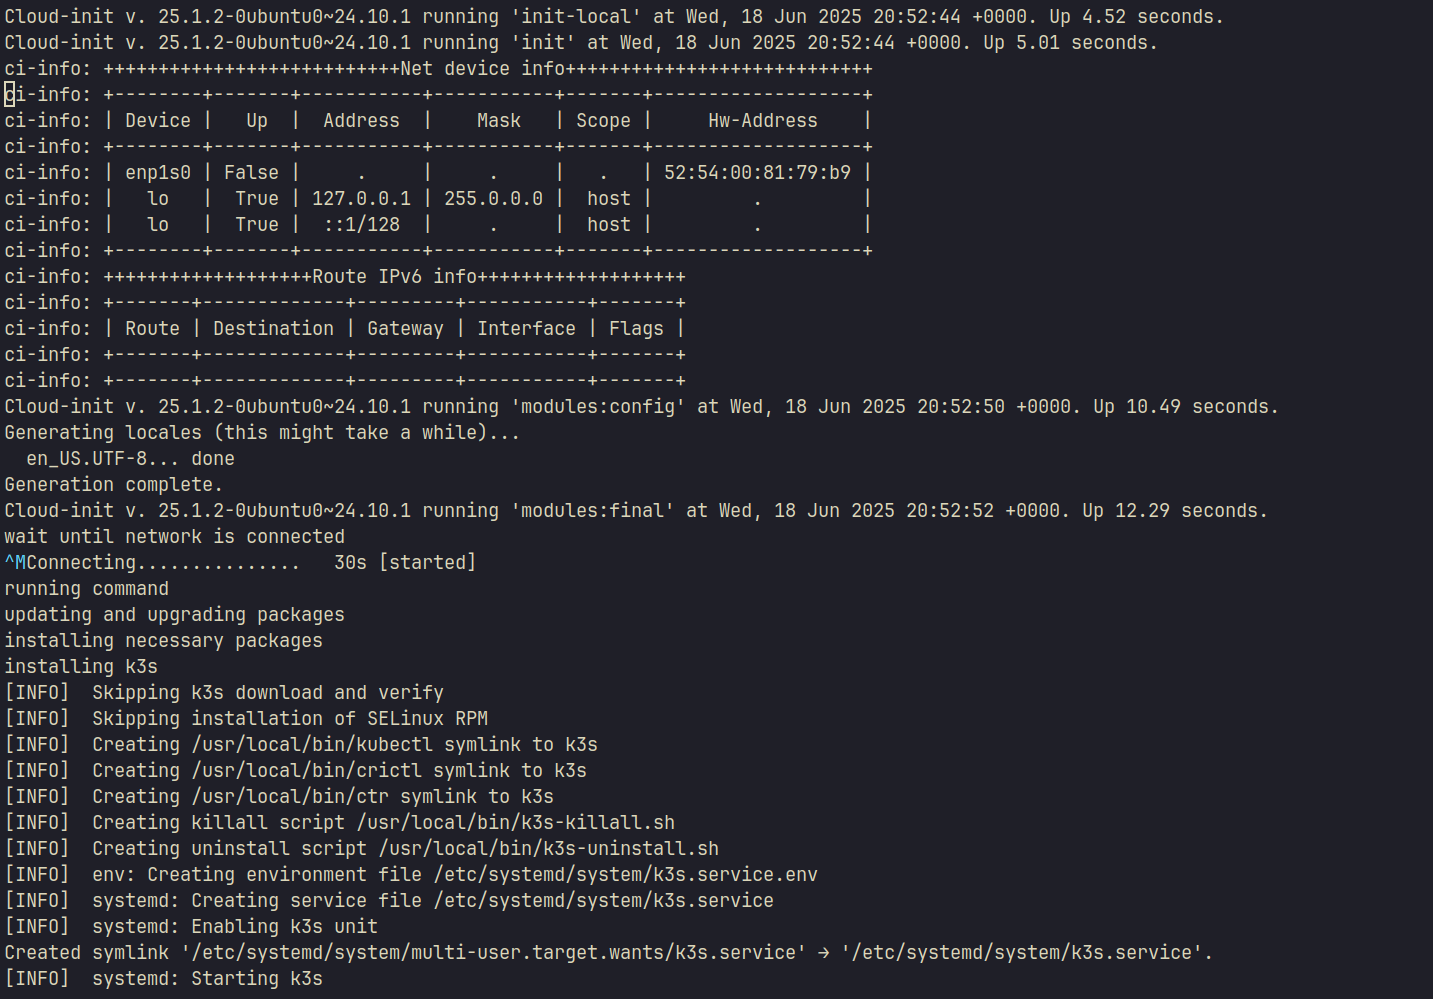
\includegraphics[scale=0.3]{gambar/cloud-init-output.png}}
  \caption{\emph{Log Command} yang Dijalankan Cloud-init}
  \label{fig:log-output-cloud-init}
\end{figure}

\subsection{\emph{Error Handling}}
\label{subsec:error-handling}

Proses \emph{provisioning virtual machine} untuk pembuatan
klaster Kubernetes tidak selalu berjalan baik. Terdapat banyak
faktor yang dapat membuat proses \emph{provisioning} gagal. Untuk
mengatasi hal tersebut, proses \emph{provisioning} pada implementasi
tugas akhir ini memiliki sifat atomik, yaitu jika terjadi \emph{error}
saat membuat \emph{virtual machine} dan \emph{virtual machine} sudah terbuat,
\emph{virtual machine} tersebut akan dihapus.

\lstinputlisting[
  language=go,
  style=codestyle,
  caption={Kode Sumber Penghapusan \emph{Virtual Machine}},
  label={lst:vm-delete-function}
]{program/delete-vm.go}

\clearpage

\lstinputlisting[
  language=go,
  style=codestyle,
  emphstyle=\color{black}\bfseries\underbar,
  emph={deleteInstance},
  caption={Contoh Penggunaan \emph{Error Handling}},
  label={lst:error-handling-example}
]{program/error-handling.go}

Pada kode sumber \ref{lst:vm-delete-function}, fungsi \lstinline{deleteInstance}
akan mematikan \emph{virtual machine} dan menghapus \emph{file} yang berkaitan
dengan \emph{virtual machine} tersebut seperti \emph{cloud image} yang dipakai.
Bentuk implementasi dari \emph{error handling} tersebut dapat dilihat pada kode
sumber \ref{lst:error-handling-example}. Pada kode sumber tersebut, jika terjadi
\emph{error} pada saat membuat \emph{virtual machine}, maka \emph{virtual machine}
tersebut akan dihapus beserta semua \emph{file} yang berkaitan.

\subsection{Mekanisme \emph{Mutex}}

Pada saat proses pembuatan VM, VM memerlukan sumber daya seperti \emph{storage}. Pada
implementasi Tugas Akhir ini, \emph{storage} yang digunakan merupakan \emph{image} file yang
akan diubah ukurannya menjadi lebih besar sesuai dengan jumlah \emph{storage} yang sudah
ditetapkan untuk setiap grup. Jika terjadi proses perubahan ukuran dari banyak
VM dalam satu waktu akan memungkinkan untuk terjadinya masalah ketika banyak VM tersebut
mencoba untuk menambah ukuran \emph{storage} dalam satu waktu yang sama.

Selain itu, VM memiliki sistem operasi tersendiri. Sumber daya yang digunakan
untuk menjalankan sistem operasi tersebut.

\section{Hasil Pengujian}
\label{sec:hasil-pengujian}

Subbab ini menjelaskan pengujian yang dilakukan pada
implementasi Tugas Akhir.

\subsection{Pengujian Pembuatan \emph{Virtual Cluster} Lingkungan Lokal}
\label{subsec:pengujian-pembuatan-vc}

Pengujian proses \emph{provisioning} pada komputer lokal bertujuan untuk
menguji apakah sistem yang telah dibangun dapat membuat \emph{virtual cluster}
yang sesuai dengan kriteria \emph{user}. Pengujian pada lingkungan lokal ini
tidak memerlukan Linux \emph{bridge} karena jaringan internet yang digunakan
oleh \emph{virtual machine} akan menggunakan \emph{Network Address Translation} (NAT)
dari \emph{host}, sehingga setiap \emph{virtual machine} dapat berkomunikasi satu sama
lain tanpa menggunakan Linux \emph{bridge}.

Skenario pengujian yang akan dilakukan pada lingkungan lokal adalah
membuat klaster Kubernetes dengan satu \emph{virtual machine} dan dua \emph{virtual machine}.
Pada klaster Kubernetes yang terdiri satu \emph{virtual machine}, \emph{virtual machine}
tersebut bertugas sebagai \emph{control plane}. Sedangkan pada klaster Kubernetes yang terdiri
dari dua \emph{virtual machine}, satu dari \emph{virtual machine} tersebut bertugas sebagai
\emph{control plane} dan sisanya sebagai \emph{worker node}.

Setelah pembuatan klaster selesai, \emph{dashboard} akan menampilkan
token untuk dapat mengakses \emph{dashboard} Kubernetes dari klaster
yang dibuat. Selain itu, tombol untuk mengakses klaster juga akan ditampilkan
dan dapat ditekan oleh \emph{user} untuk menuju situs web \emph{dashboard}
klaster Kubernetes.

\begin{figure}[H]
  \centering
  \fbox{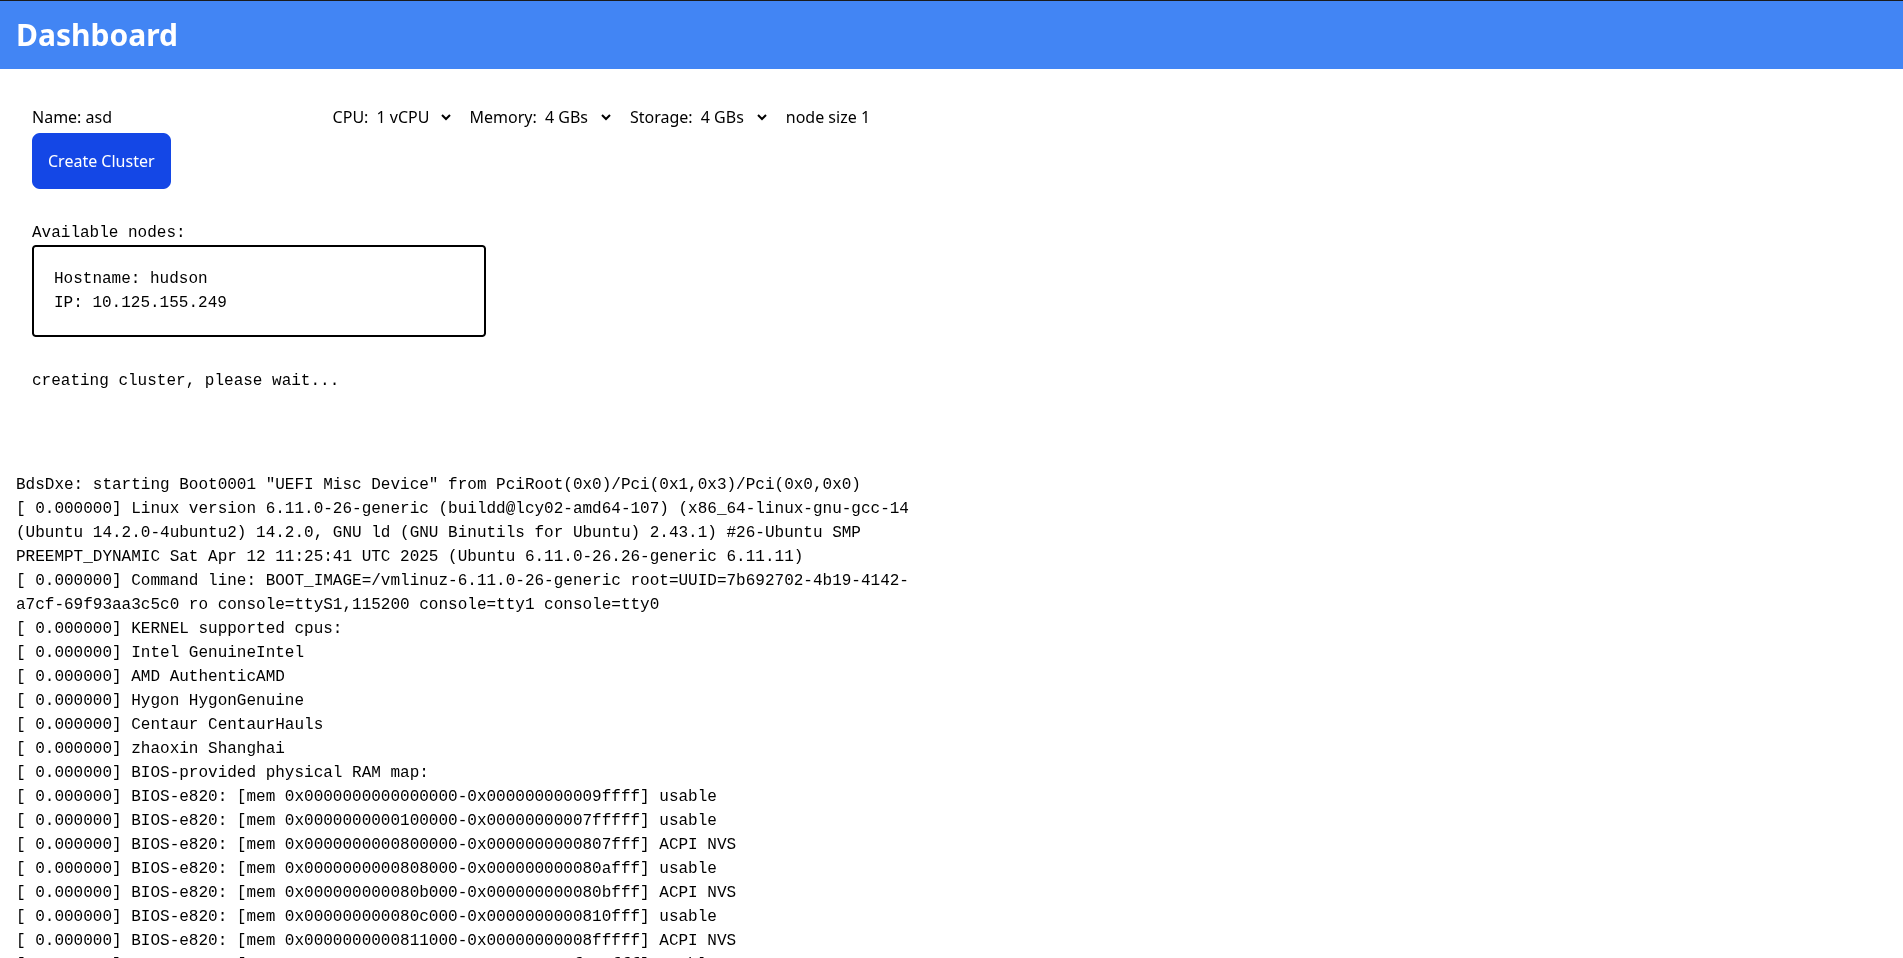
\includegraphics[scale=0.3]{gambar/website-create-process.png}}
  \caption{Proses Pembuatan Klaster}
  \label{fig:proses-pembuatan-klaster}
\end{figure}

\begin{figure}[H]
  \centering
  \fbox{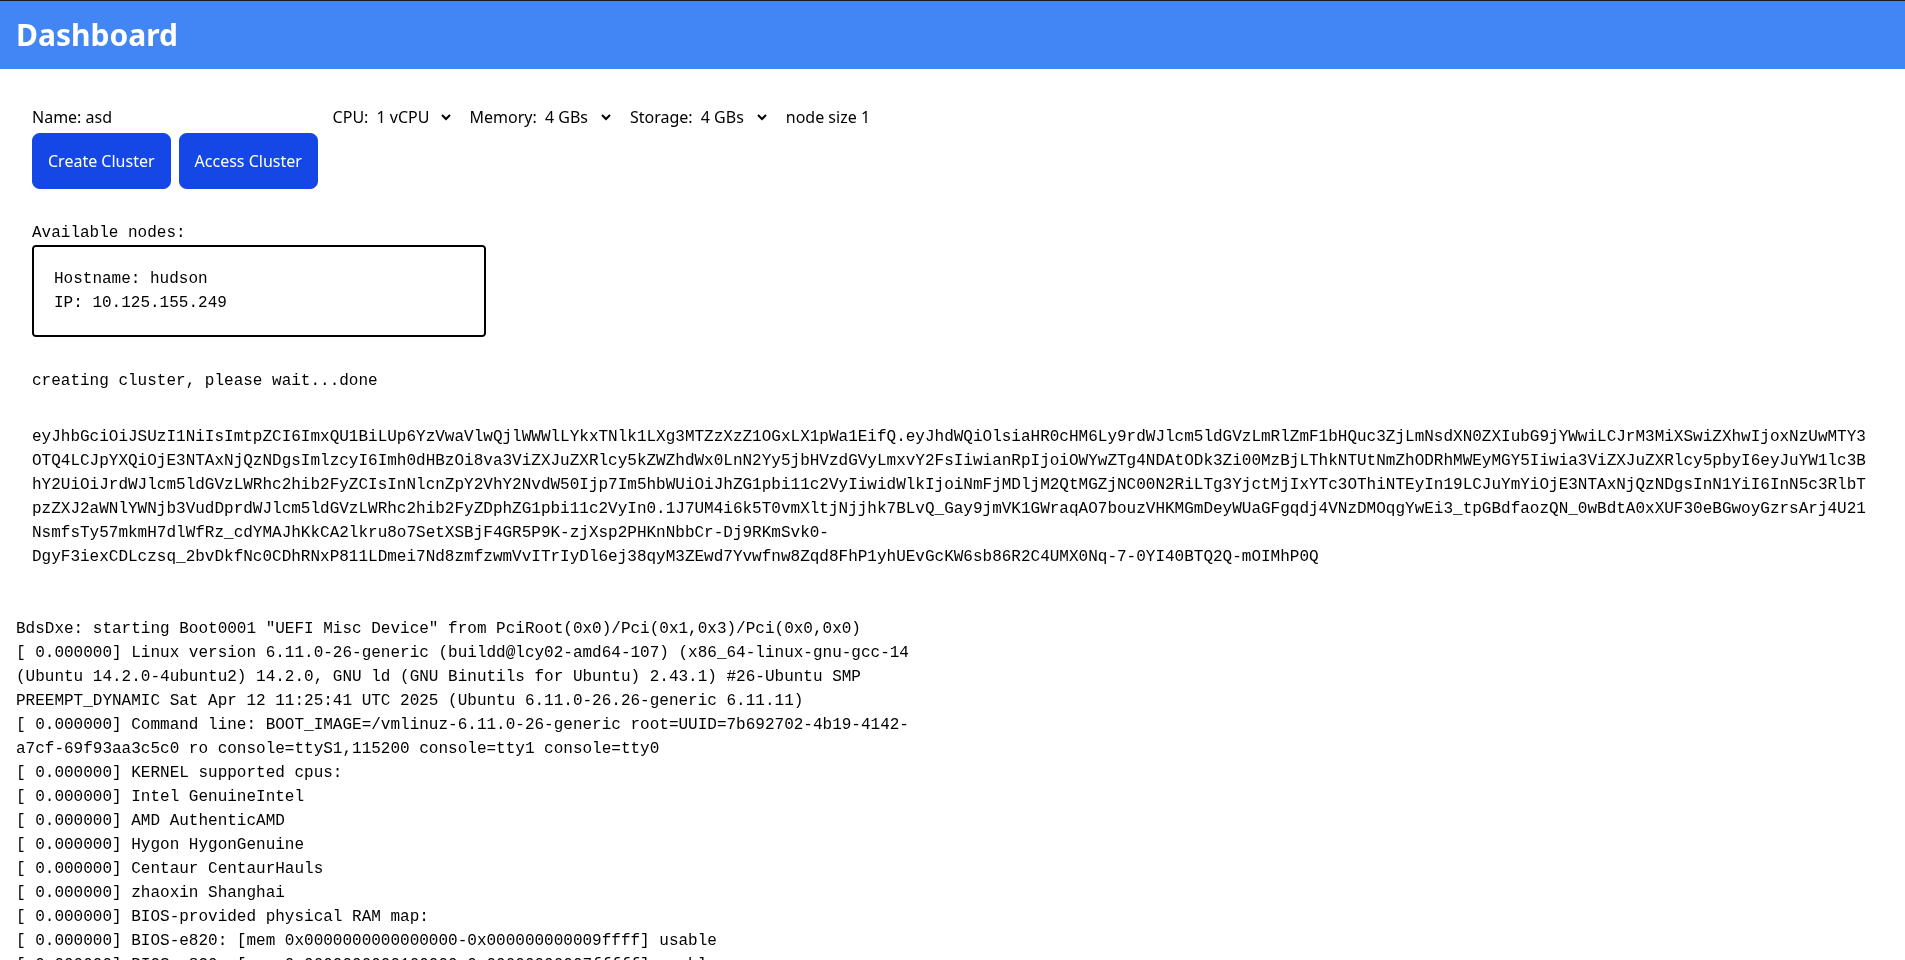
\includegraphics[scale=0.3]{gambar/website-create-process-done-local.png}}
  \caption{Proses Pembuatan Klaster Selesai}
  \label{fig:proses-pembuatan-klaster-selesai}
\end{figure}

\begin{figure}[H]
  \centering
  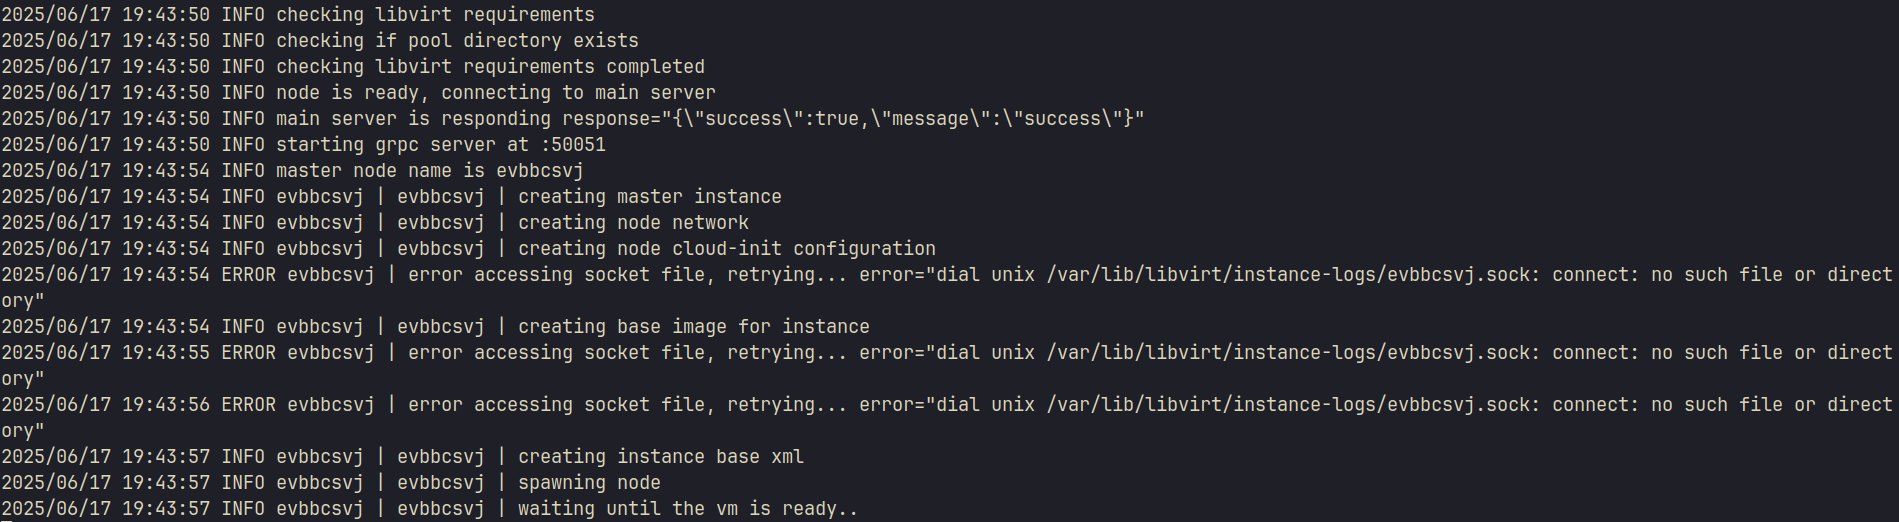
\includegraphics[scale=0.3]{gambar/worker-create-cluster-process-local.png}
  \caption{\emph{Log} pada Komputer \emph{Worker}}
  \label{fig:worker-create-cluster-process-local}
\end{figure}

\begin{figure}[H]
  \centering
  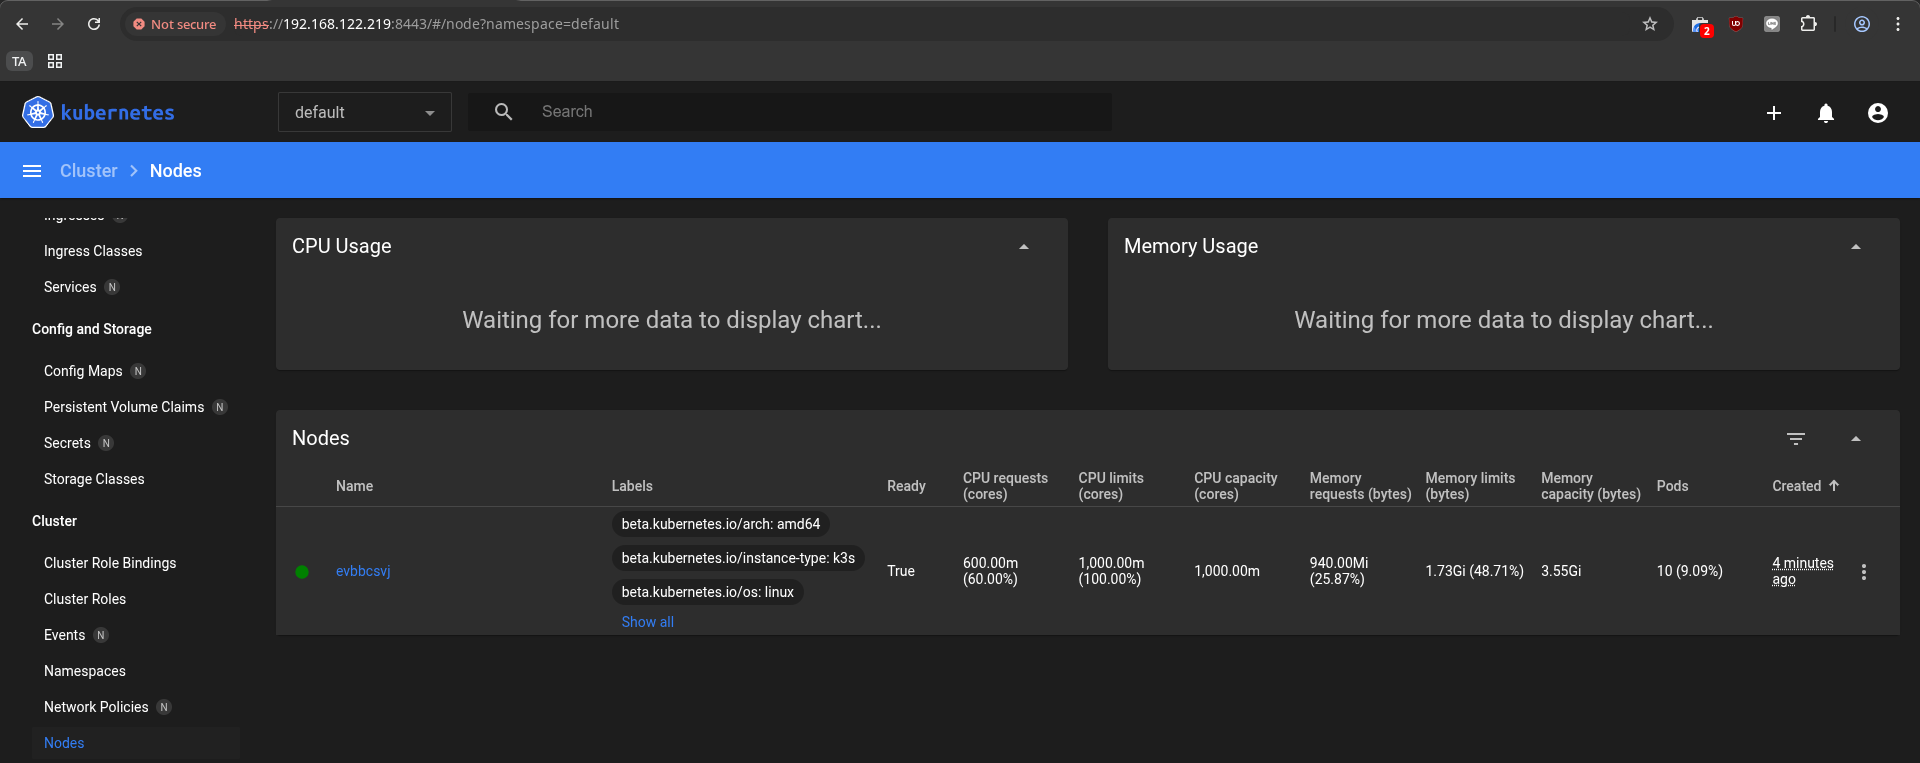
\includegraphics[scale=0.3]{gambar/kubernetes-dashboard-access-local-with-nodes.png}
  \caption{Daftar \emph{Nodes} pada Klaster dengan Satu \emph{Virtual Machine}}
  \label{fig:daftar-nodes-pada-dashboard-kubernetes}
\end{figure}

Berdasarkan gambar-gambar di atas, sistem \emph{provisioning} dapat membuat
\emph{virtual machine} yang secara otomatis tergabung dalam sebuah klaster Kubernetes.
Selain itu, \emph{control plane} juga menyediakan \emph{dashboard} Kubernetes yang dapat
digunakan oleh pengguna untuk berinteraksi dengan klaster Kubernetes tersebut.

\subsection{Pengujian Pembuatan \emph{Virtual Cluster} Lingkungan \emph{Production}}
\label{subsec:pengujian-pembuatan-vc-prod}

Pada lingkungan \emph{production}, \emph{virtual machine} yang tergabung dalam
satu klaster tidak selalu berada dalam satu komputer fisik \emph{worker} yang sama.
Pengujian dilakukan dengan cara membuat klaster berisi dua atau lebih \emph{virtual machine}
yang terdiri dari satu \emph{control plane} dan sisanya sebagai \emph{worker node}.
Semua \emph{Virtual machine} tersebut tidak selalu berada di komputer \emph{worker}
yang sama.

Pada subbab pengujian ini, akan dibuat sebuah klaster yang terdiri dari dua
\emph{virtual machine} yang berada di dua komputer fisik yang berbeda. Pada gambar
\ref{fig:nodes-2-komputer-berbeda-1}, klaster tersebut memiliki \emph{nodes} yang
bernama eovugekt dan gxlshrqm. Komputer fisik dari dua \emph{virtual machine}
tersebut dapat dilihat pada gambar \ref{fig:vm-komputer-fisik-1}.

Gambar \ref{fig:vm-komputer-fisik-1} menunjukkan bahwa \emph{nodes} gxlshrqm berada
pada komputer fisik rpl-1 dan \emph{nodes} eovugekt berada pada
komputer fisik rpl-02. Untuk pengujian \emph{multi-tenancy}, akan
dibuat klaster Kubernetes lagi dari dua komputer fisik tersebut.

Pada gambar \ref{fig:nodes-2-komputer-berbeda-2}, klaster yang baru
memiliki \emph{nodes} bernama qxwuyusc dan vsbftqms. Gambar \ref{fig:vm-komputer-fisik-2}
menunjukkan bahwa \emph{node} qxwuyusc berada pada komputer fisik rpl-02 yang juga
merupakan komputer fisik dari \emph{node} eovugekt. Dari hal tersebut, dapat
dilihat bahwa komputer fisik rpl-02 digunakan oleh dua klaster dan dua pengguna
yang berbeda.

\begin{figure}[H]
  \centering
  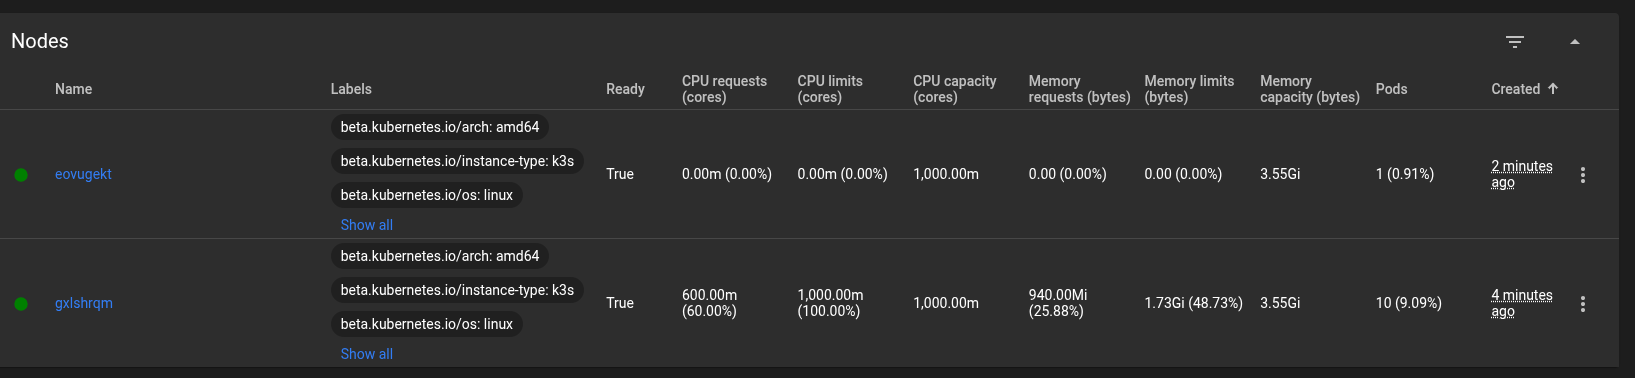
\includegraphics[scale=0.3]{gambar/two-nodes-difference-computer-dashboard.png}
  \caption{Daftar \emph{Nodes} pada Klaster 1}
  \label{fig:nodes-2-komputer-berbeda-1}
\end{figure}

\begin{figure}[H]
  \centering
  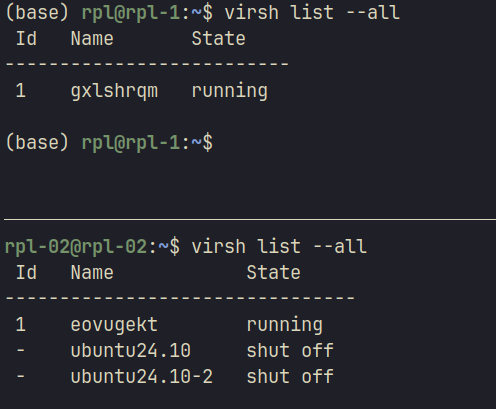
\includegraphics[scale=0.3]{gambar/ssh-nodes-list-1.png}
  \caption{Daftar \emph{Virtual Machine} Setelah Pembuatan Klaster 1}
  \label{fig:vm-komputer-fisik-1}
\end{figure}

\begin{figure}[H]
  \centering
  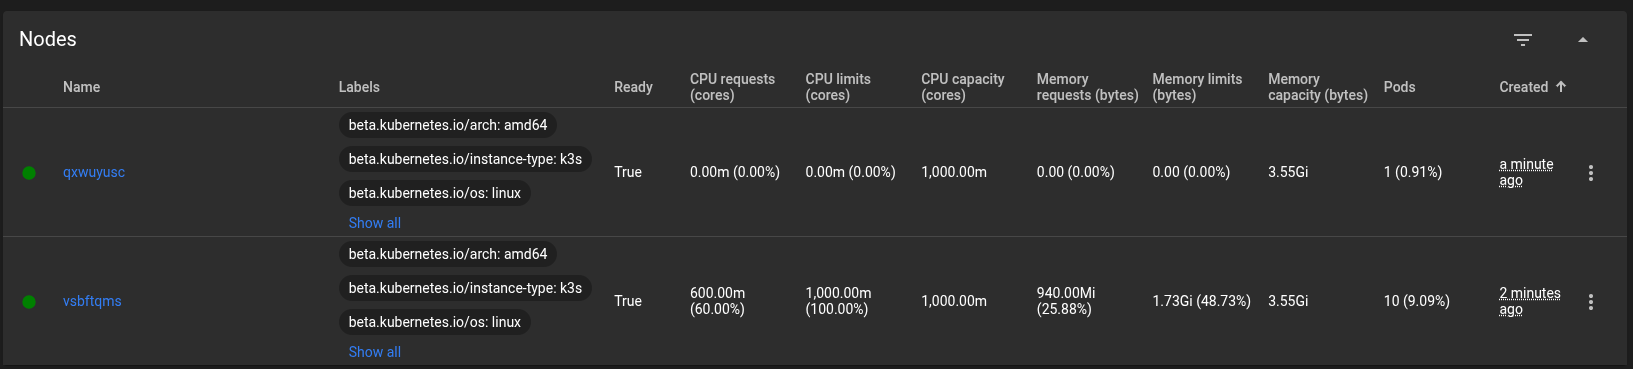
\includegraphics[scale=0.3]{gambar/two-nodes-difference-computer-dashboard-2.png}
  \caption{Daftar \emph{Nodes} pada Klaster 2}
  \label{fig:nodes-2-komputer-berbeda-2}
\end{figure}

\begin{figure}[H]
  \centering
  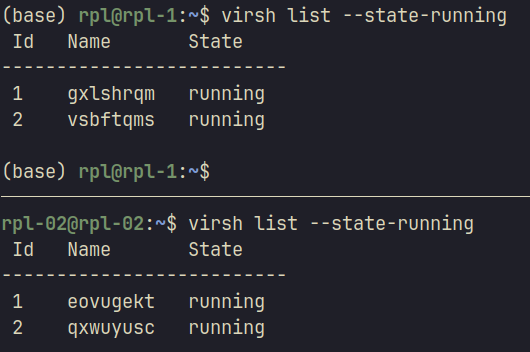
\includegraphics[scale=0.3]{gambar/ssh-nodes-list-2.png}
  \caption{Daftar \emph{Virtual Machine} Setelah Pembuatan Klaster 2}
  \label{fig:vm-komputer-fisik-2}
\end{figure}

\subsection{Pengujian \emph{Deployment} pada Klaster Kubernetes}
\label{subsec:pengujian-deployment}

Pengujian berupa \emph{Deployment} pada Klaster Kubernetes dilakukan dengan
menggunakan Nginx yang akan diekspos. Kemudian memeriksa apakah \emph{Deployment}
tersebut dapat diakses atau tidak. \emph{Command line} yang digunakan untuk
membuat \emph{Deployment} Nginx kemudian mengekspos agar dapat diakses
dapat dilihat pada \ref{cli:cli-deployment-nginx}.

{\renewcommand{\lstlistingname}{Instruksi Terminal}
\begin{lstlisting}[
  style=clistyle,
  caption={\emph{Command Line} untuk Membuat \emph{Deployment} Nginx},
  label={cli:cli-deployment-nginx},
]
$ kubectl create deployment nginx --image=nginx
deployment.apps/nginx created

$ kubectl expose deployment nginx --type=NodePort --port=80 --target-port=80
service/nginx exposed

$ kubectl get svc nginx
NAME    TYPE       CLUSTER-IP   EXTERNAL-IP   PORT(S)        AGE
nginx   NodePort   10.43.5.58   <none>        80:32673/TCP   14s
\end{lstlisting}
}

Berdasarkan instruksi terminal \ref{cli:cli-deployment-nginx}, \emph{Deployment}
Nginx pada klaster tersebut diekspos ke \emph{port} 32673. Hasil pengaksesan
\emph{Deployment} tersebut dapat dilihat pada gambar \ref{fig:nginx-deployment}.
Dapat dilihat juga pada gambar \ref{fig:nginx-deployment} bahwa \emph{port} yang diakses adalah
\emph{port} 32673.

\begin{figure}[H]
  \centering
  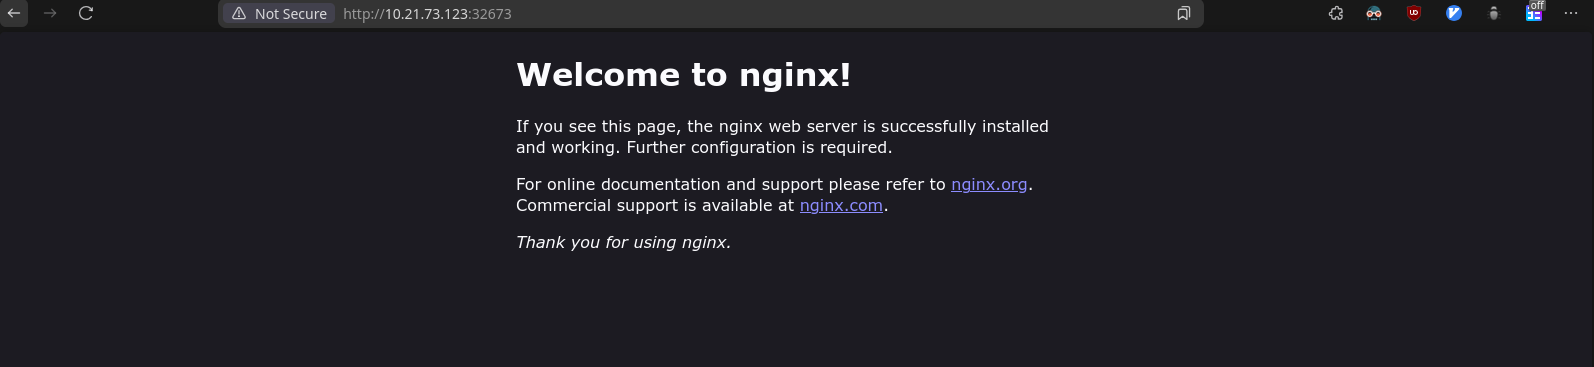
\includegraphics[scale=0.3]{gambar/nginx-deployment.png}
  \caption{Halaman Situs Web Nginx \emph{Deployment} pada Klaster}
  \label{fig:nginx-deployment}
\end{figure}

\subsection{Pengujian Waktu Pembuatan Klaster Kubernetes}
\label{subsec:pengujian-deployment}

Pengujian ini dilakukan untuk mengetahui waktu yang diperlukan untuk membuat
klaster Kubernetes dengan beberapa variabel yang berbeda seperti berikut:

\begin{itemize}

  \item[-] 1 \emph{worker}
  
  \item[-] 2 \emph{worker}

  \item[-] 3 \emph{worker}

\end{itemize}

Untuk semua percobaan dengan variabel yang sudah disebutkan sebelumnya, jumlah \emph{virtual cluster}
yang dibuat adalah 5 dengan masing-masing \emph{virtual cluster} terdiri dari 2 \emph{node}
dan tiap \emph{node} memiliki 2 VCPU, 2 GB \emph{memory}, dan 4 GB \emph{storage}. Ketentuan
sumber daya tersebut berdasarkan sumber daya minimum yang dibutuhkan oleh K3s dalam menjalankan
klaster, yaitu \emph{control plane} dengan 2 \emph{cores} CPU dan 2GB RAM, dan \emph{node}
dengan 1 \emph{core} CPU dan 512MB RAM. K3s tidak menyebutkan ukuran penyimpanan minimum yang dibutuhkan
untuk menjalankan klaster, sehingga penentuan ukuran penyimpanan berdasarkan pada ukuran penyimpanan
minimum untuk Ubuntu \emph{cloud image}, yaitu 4GB. Selain itu, ukuran penyimpanan yang besar akan
membuat proses \emph{provisioning} VM membutuhkan waktu yang lebih lama, terlebih lagi jika perangkat
keras untuk penyimpanan tidak menggunakan \emph{Solid State Drive} (SSD) dan masih menggunakan
\emph{Hard Disk Drive} (HDD). Tabel waktu yang diperlukan untuk menyelesaikan \emph{job}
pembuatan 5 \emph{virtual cluster} dapat dilihat pada tabel \ref{tb:test-1-worker}, \ref{tb:test-2-worker},
dan \ref{tb:test-3-worker}.

\begin{longtable}{|c|c|}
  \caption{Waktu yang Dibutuhkan Menggunakan 1 \emph{Worker}}
  \label{tb:test-1-worker}                                   \\
  \hline
  \rowcolor[HTML]{C0C0C0}
  \textbf{Percobaan} & \textbf{Waktu Total yang Dibutuhkan} \\
  \hline
  1            & 14 menit 40 detik \\
  2            & 11 menit  0 detik \\
  3            & 12 menit 30 detik \\
  4            & 15 menit  5 detik \\
  5            & 14 menit 15 detik \\
  \hline
  \textbf{Rata-Rata} & \textbf{13 Menit 30 detik} \\
  \hline
\end{longtable}

\begin{longtable}{|c|c|}
  \caption{Waktu yang Dibutuhkan Menggunakan 2 \emph{Worker}}
  \label{tb:test-2-worker}                                   \\
  \hline
  \rowcolor[HTML]{C0C0C0}
  \textbf{Percobaan} & \textbf{Waktu Total yang Dibutuhkan} \\
  \hline
  1 &  9 menit  5 detik \\
  2 &  9 menit 50 detik \\
  3 & 13 menit  0 detik \\
  4 &  9 menit 35 detik \\
  5 & 11 menit 50 detik \\
  \hline
  \textbf{Rata-Rata} & \textbf{10 Menit 40 detik} \\
  \hline
\end{longtable}

\begin{longtable}{|c|c|}
  \caption{Waktu yang Dibutuhkan Menggunakan 3 \emph{Worker}}
  \label{tb:test-3-worker}                                   \\
  \hline
  \rowcolor[HTML]{C0C0C0}
  \textbf{Percobaan} & \textbf{Waktu Total yang Dibutuhkan} \\
  \hline
  1 & 11 menit 50 detik \\
  2 &  9 menit 15 detik \\
  3 &  8 menit 45 detik \\
  4 &  9 menit 30 detik \\
  5 &  9 menit 45 detik \\
  \hline
  \textbf{Rata-Rata} & \textbf{9 Menit 49 detik} \\
  \hline
\end{longtable}

Dalam proses pengujian, 5 permintaan pembuatan \emph{virtual cluster}
tersebut terjadi dalam satu waktu. Semua permintaan pembuatan tersebut
akan dimasukkan ke dalam \emph{queue} yang kemudian akan dikerjakan oleh
\emph{worker}.

Pada saat \emph{worker} mengerjakan permintaan pembuatan \emph{virtual cluster},
\emph{worker} akan mengirim permintaan tersebut ke \emph{worker node}
secara \emph{random}. \emph{List} dari \emph{worker node} yang digunakan
dalam proses pengujian ini dapat dilihat pada gambar \ref{fig:testing-worker-nodes}.
Berdasarkan tabel waktu total yang dibutuhkan untuk menyelesaikan
semua permintaan, rata-rata waktu yang dibutuhkan untuk menyelesaikan semua permintaan
tersebut menjadi lebih cepat ketika \emph{worker} yang digunakan meningkat.
Namun, total waktu yang dibutuhkan untuk menyelesaikan semua permintaan
tersebut tidak selalu lebih cepat ketika menggunakan \emph{worker} yang lebih banyak.
Salah satu contohnya adalah percobaan 3 dengan 2 \emph{worker}. Waktu yang
dibutuhkan adalah 13 menit 0 detik. Pada beberapa percobaan dengan menggunakan
hanya 1 \emph{worker}, percobaan 2 menghasilkan waktu 11 menit 0 detik. Hal tersebut
dapat terjadi jika \emph{worker node} yang sama dipilih pada saat percobaan 3 dengan 2 \emph{worker}

\begin{figure}[H]
  \centering
  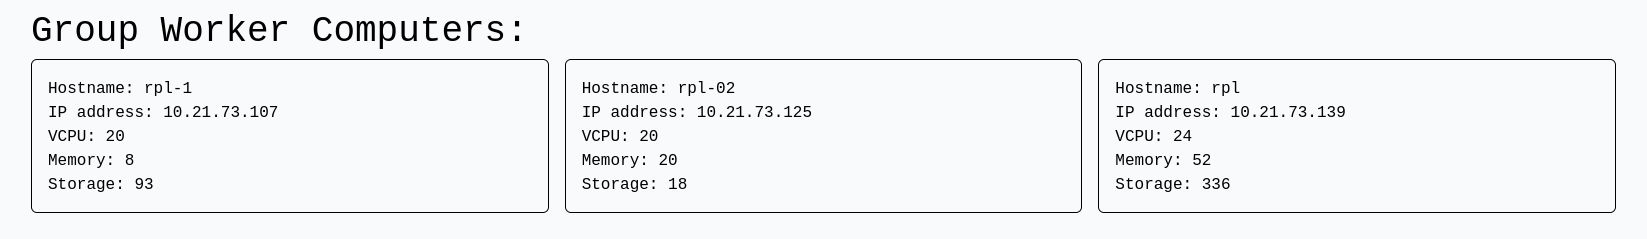
\includegraphics[scale=0.365]{gambar/testing-workers.png}
  \caption{\emph{Worker Node} yang Digunakan untuk Pengujian.}
  \label{fig:testing-worker-nodes}
\end{figure}

% Contoh pembuatan tabel
% \begin{longtable}{|c|c|c|}
%   \caption{Hasil Pengukuran Energi dan Kecepatan}
%   \label{tb:EnergiKecepatan}                                   \\
%   \hline
%   \rowcolor[HTML]{C0C0C0}
%   \textbf{Energi} & \textbf{Jarak Tempuh} & \textbf{Kecepatan} \\
%   \hline
%   10 J            & 1000 M                & 200 M/s            \\
%   20 J            & 2000 M                & 400 M/s            \\
%   30 J            & 4000 M                & 800 M/s            \\
%   40 J            & 8000 M                & 1600 M/s           \\
%   \hline
% \end{longtable}
